\begin{surferPage}[Septica-Labs]{O septic\u{a} cu 99 de singularit\u{a}\c{t}i}
     Oliver Labs a construit o suprafa\c{t}\u{a} de grad $7$ (septic\u{a}) \^{i}n timp ce lucra la
    dizerta\c{t}ia lui la Universitatea din Mainz, \^{i}n 2004. Acesta este recordul mondial actual
    de grad $7$. Dar nu este exclus s\u{a} existe o suprafa\c{t}\u{a} septic\u{a} cu $104$ singularit\u{a}\c{t}i!
    Suprafa\c{t}a lui Labs are simetria unui heptagon regulat (imaginea din st\^{a}nga).
    Acest lucru este vizibil c\^{a}nd privim suprafa\c{t}a de sus (imaginea din dreapta):

    \vspace*{-0.3em}
    \begin{center}
      \begin{tabular}{c@{\qquad}c}
        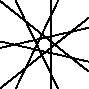
\includegraphics[height=1.5cm]{./../../common/images/labsseptic1.pdf}
        &
        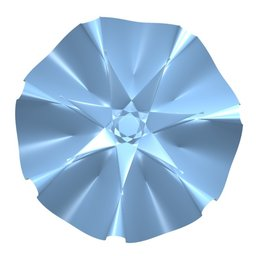
\includegraphics[height=1.5cm]{./../../common/images/labs_septic_von_oben}
      \end{tabular}
    \end{center}
    \vspace*{-0.3em}

    Pentru construirea acestei suprafe\c{t}e, Oliver Labs a folosit sistemul informatic
    {\sc Singular} (Universitatea Kaiserslautern), care este foarte potrivit pentru
    calcule \^{i}n geometria algebric\u{a} \c{s}i singularit\u{a}\c{t}i.

    El a folosit aritmetica modular\u{a}. Un exemplu de acest lucru ar fi un ceas: \c{s}tim c\u{a} 24:00$=$0:00,
    iar ora 24:00$+$ 1 nu este ora 25:00, ci ora 1:00.
\end{surferPage}
